\documentclass{parcfd}

\usepackage{graphicx}
\usepackage{subcaption}
\usepackage{amsmath}
\usepackage{amsfonts}
\usepackage{amssymb}

\graphicspath{{figures/}}

\title{REPLICATION STUDIES AND REPRODUCIBILITY CHECKLIST FOR COMPUTATIONAL FLUID DYNAMICS}

\author{Lorena A. BARBA$^{*}$ AND Olivier MESNARD$^{*}$}

\heading{Lorena A. Barba and Olivier Mesnard}

\address{$^{*}$ The George Washington University\\
Department of Mechanical \& Aerospace Engineering\\
20052 Washington DC, USA\\
e-mail: labarba@gwu.edu, web page: http://lorenabarba.com}

\keywords{Reproducibility, Replicability, Parallel CFD applications, Immersed boundary method, Singularity containerization, Reproducibility checklist}

\abstract{We conduct replication studies our previously published computational studies with our in-house research code to highlight sources of non-reproducibility in Computational Fluid Dynamics. Our objective is to develop guidance on what computational artifacts and what level of detail need to be shared for reproducibility and replication to be possible. We design a reproducibility checklist tailored for CFD that could be used by journals and conferences.}

\begin{document}
%\maketitle

\section{INTRODUCTION}

We rely on computer simulations and data models to create new knowledge.
But how much evidence do we need to provide to assert the veracity of the new scientific findings claimed in published manuscript or in a conference talk?
Published studies rarely come with the underlying software and computational steps that we used to produce the results.
Starting from the fact that software contain bugs and that published manuscripts are not free of typos, if researchers do not make their code and data available, there is little hope of knowing how data were processed and if it was the right thing to do.

In 2019, the National Academies of Sciences, Engineering, and Medicine released a consensus report \cite{nasem_2019} that provides findings and recommendations for improving rigor and transparency in research.
The report also gives clear definitions of ``reproducibility'' and ``replicability'' that are intended to apply across all fields of science.

\begin{itemize}
    \item[-] Reproducibility is obtaining consistent results using the same input data; computational steps, methods, and code; and conditions of analysis.
    \item[-] Replicability is obtaining consistent results across studies aimed at answering the same scientific question, each of which had obtained its own data. Two studies may be considered to have replicated if they obtain consistent results given the level of uncertainty inherent in the system under study.
\end{itemize}

In the past, we have attempted to replicate our own results.
The outputs of this replication study have been published in \cite{mesnard_barba_2017}, in which we also reported the many obstacles faced.
Knowing how challenging it was to replicate our own results, we now want to estimate how much effort it takes to replicate the computational results from other research groups.

Objectives are (1) investigate causes of non-reproducibility in computational fluid dynamics applications, particularly in HPC situations; (2) conduct replication of previously published computational results, looking to identify sources of non-replicability; (3) develop guidance on what computational artifacts and what level of detail need to be shared for reproducibility and replication to be possible; (4) design workflows for computational research to guarantee, as much as possible, that findings are both reproducible and replicable.

\section{REPLICATION STUDIES}

We use our in-house research software, called PetIBM, to conduction replication of two previously published computational results: a new formulation of the immersed boundary method and a study on the wake topology and propulsive performance of pitching-rolling wings.
Since the computational code, input data, and conditions of analysis used to produce the original numerical results are not made available, we consider the two studies to be not reproducible.
But, can we replicate the scientific findings? And can we do it in a reproducible way?

\subsection{Reproducible workflow}

PetIBM \cite{chuang_et_al_2018} is an open-source research code that solved the incompressible Navier-Stokes equations with a projection method (framed as a block-LU decomposition) on structure Cartesian grids, with an immersed boundary method (IBM) to compute the flow around immersed bodies.
PetIBM relies on the data structures and parallel routines of the PETSc library to run on distributed-memory architectures, with the capability to solve linear systems on multiple GPU devices distributed across the nodes, with the NVIDIA AmgX library.
The software is open source, version-controlled with Git, hosted on GitHub, shared under the permissive 3-clause BSD license, and archived on Zenodo.

To capture the conditions analysis, we use the container technologies of Docker and Singularity.
We have already used Docker containers in the past to create a reproducible workflow on the public cloud provider Microsoft Azure \cite{mesnard_barba_2020}.
Here, we adopt a similar reproducible workflow to conduct numerical simulations on a University-managed HPC cluster.
However, Docker is not available at most HPC centers for security reasons; the Docker daemon requires root privileges that users do not have on shared production clusters.
An alternative to Docker at HPC centers is the container technology of Singularity, which was designed from the ground up to prevent escalation of user privileges.
Singularity images used to produce the results of a computational study are made publicly available on the registry SingularityHub.
Researchers interested in reproducing our results can pull the images to create a faithfully reproduced computational environment.

\subsection{Decoupled immersed boundary projection method}

Taira \& Colonius \cite{taira_colonius_2007} proposed the immersed boundary projection method (IBPM) where the divergence-free constraint and the no-slip condition for the velocity field are simultaneously enforced at each time step.
The method requires to solve an expensive modified Poisson system for the pressure field and boundary forces, grouped together.
Li and co-authors \cite{li_et_al_2016} proposed to apply an additional block-LU decomposition to decouple the variables and retrieve a classical pressure Poisson system.
However, the constraints are not anymore satisfied simultaneously.
The authors of the decoupled IBPM suggested several algorithms and schemes that differs by the order in which the constraints are enforced.

We have implemented the different algorithms of the decoupled IBPM in an open-source PetIBM application code that is version-controlled and hosted on GitHub, and shared under the 3-clause BSD license.
This replication study highlights discrepancies in the numerical results when re-implementing the ``same'' algorithm (Figure \ref{fig:cylinder2dRe40:pressure_coefficient}).

\begin{figure}
    \centering
    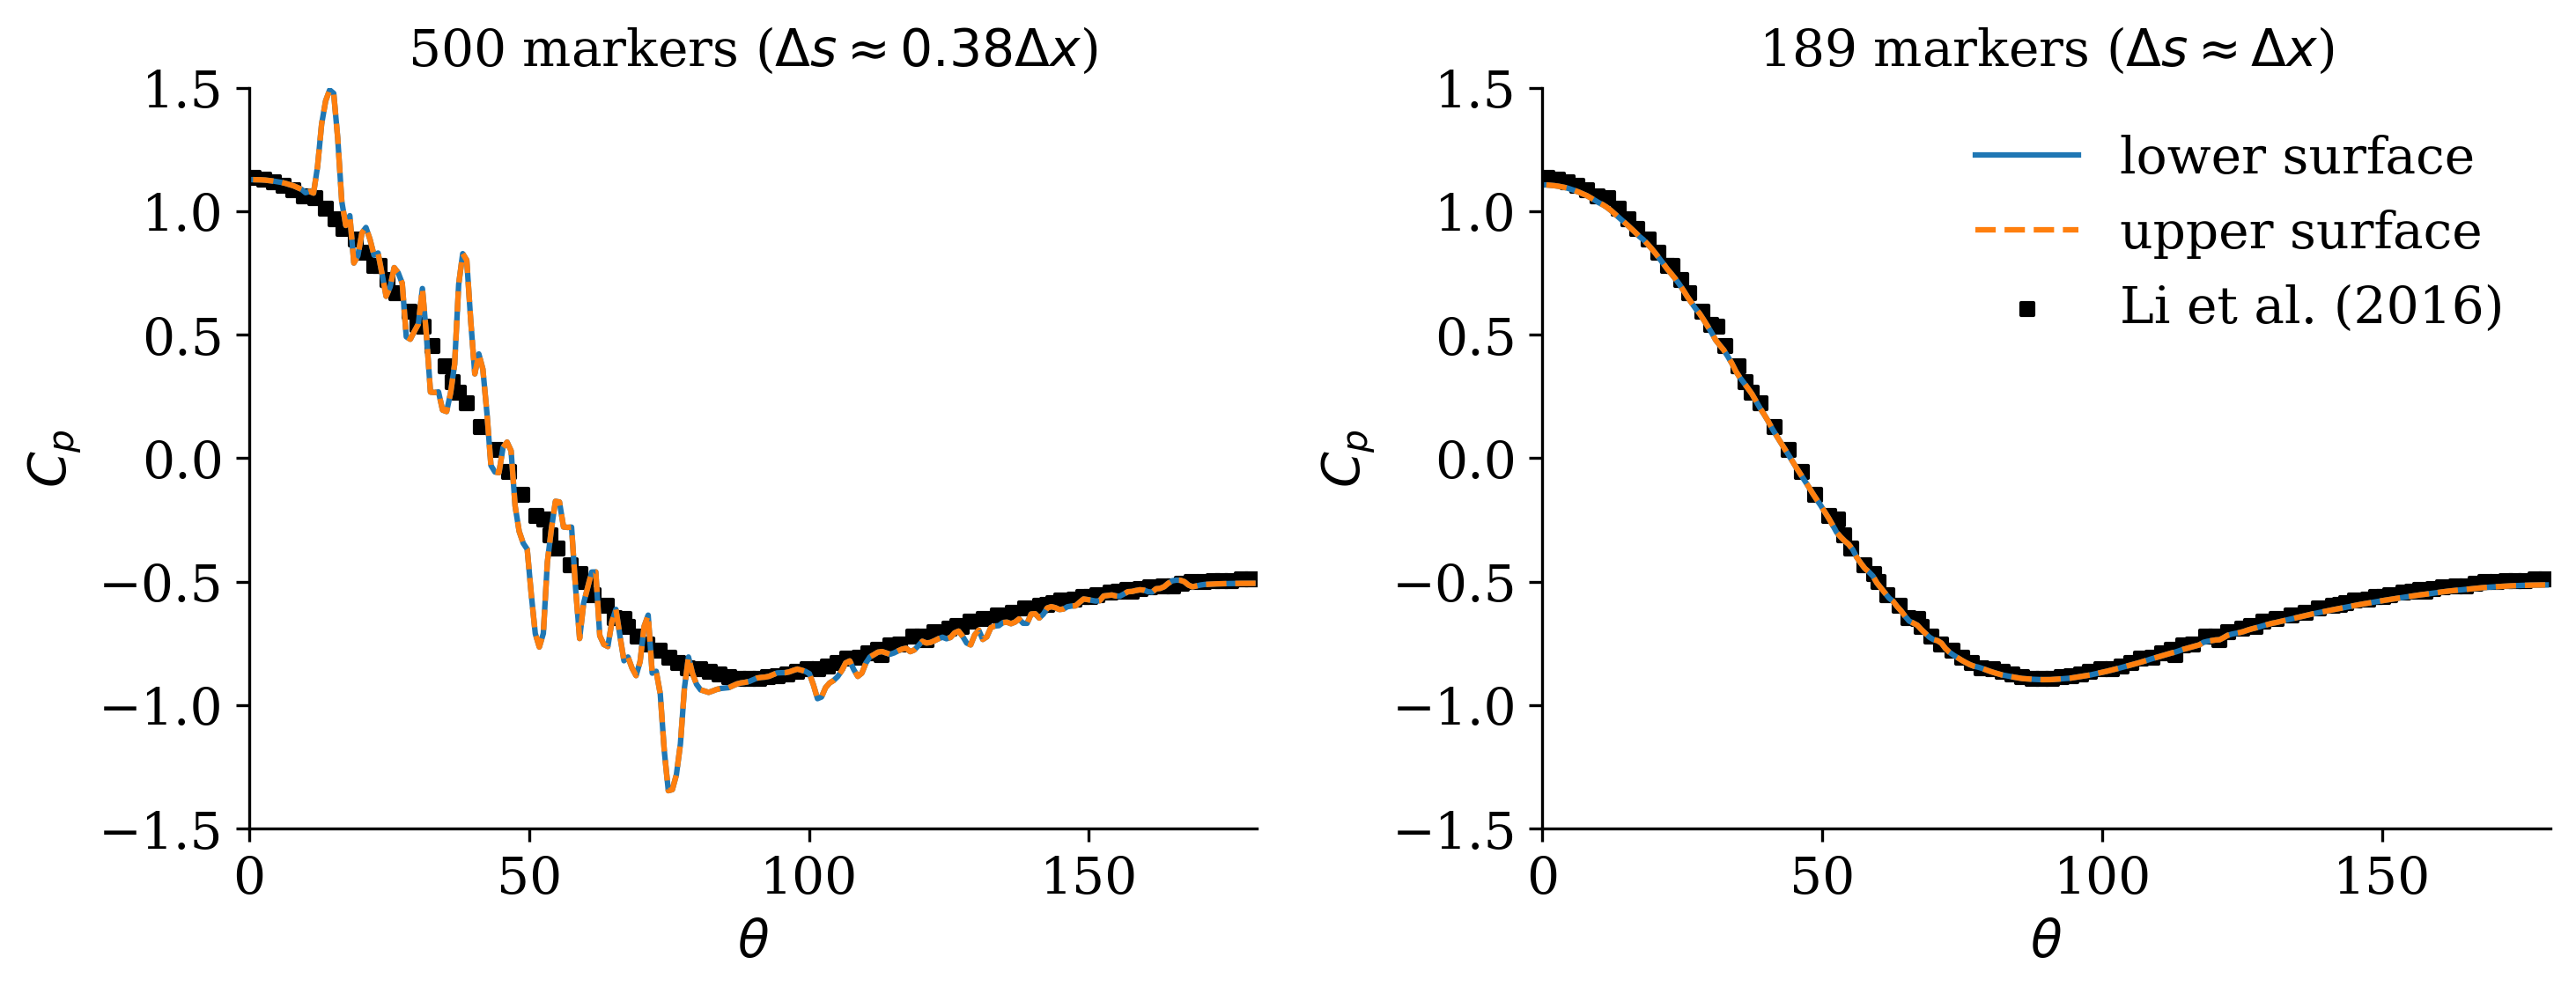
\includegraphics[width=\linewidth]{cylinder2dRe40_pressure_coefficient.png}
    \caption{Distribution of the pressure coefficient along the surface of a stationary cylinder at Reynolds number $Re = 40$. With PetIBM, we used two different resolutions to discretize the immersed boundary: (left) $500$ equally spaced markers as in the original study \cite{li_et_al_2016} and (right) $189$ markers to maintain a similar resolution between the Lagrangian surface mesh and Eulerian grid.}
    \label{fig:cylinder2dRe40:pressure_coefficient}
\end{figure}

\subsection{Wake topology of low-aspect-ratio pitching-rolling plates}

Many prior studies have focused on the pitching and heaving motion of three-dimensional wings, but only few studies have focused on the rolling and pitching motion, which could serve as a better canonical model for investigating the hydrodynamics of bio-inspired flapping propulsion.
Li \& Dong \cite{li_dong_2016} conducted a parametric study for the rolling-pitching motion to quantify the wake topology and propulsive performance of low-aspect ratio elliptical wings.
They used their own research code to produce the numerical results, which implements a different immersed-boundary method (sharp-interface technique with a ghost-cell methodology) that those implemented in PetIBM (diffused-interface method through regularized delta functions).

We have implemented the three-dimensional rolling and pitching kinematics (Figure \ref{fig:rollingpitching}) in an open-source PetIBM application code, hosted on GitHub and shared under the 3-clause BSD license.
We aim at replicating the scientific findings with out code base and highlight possible differences in the results that may com from the use of a different immersed-boundary technique.

\begin{figure}
    \centering
    \begin{subfigure}{0.4\textwidth}
        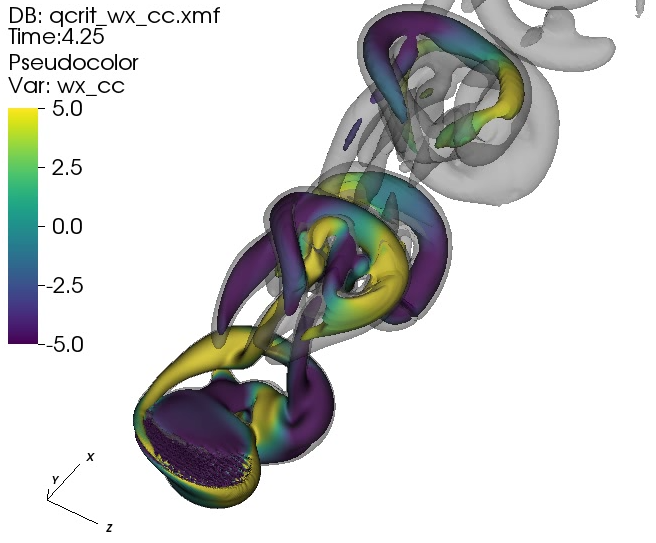
\includegraphics[width=\linewidth]{rollingpitching_perspective.png}
        \caption{}
        \label{fig:rollingpitching:perspective}
    \end{subfigure}
    \hspace*{1cm}
    \begin{minipage}{0.3\textwidth}
        \begin{subfigure}{\linewidth}
            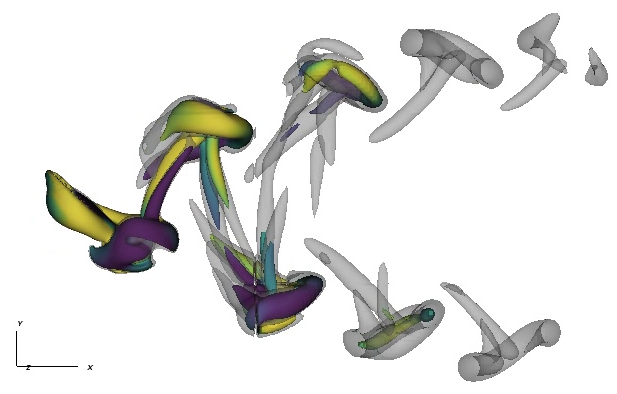
\includegraphics[width=\linewidth]{rollingpitching_side_view.png}
            \caption{}
            \label{fig:rollingpitching:side_view}
        \end{subfigure}
        \vspace*{1cm}
        \begin{subfigure}{\linewidth}
            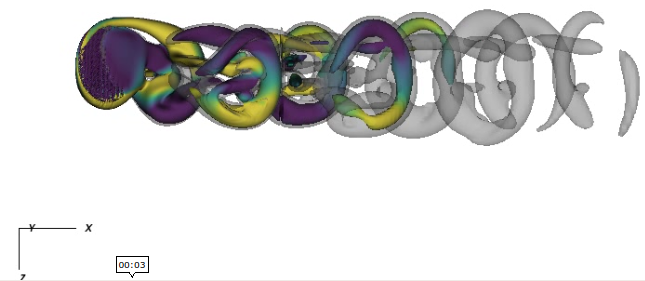
\includegraphics[width=\linewidth]{rollingpitching_top_view.png}
            \caption{}
            \label{fig:rollingpitching:top_view}
        \end{subfigure}
    \end{minipage}
    \caption{Wake topology of a pitching and rolling circular plate after four flapping cycles at Reynolds number $Re = 200$ and Strouhal number $St = 0.6$. Flow structures are visualized using the Q-criterion for $Q = 1$ (colored by the streamwise vorticity) and $Q = 6$ (gray). (a) Perspective view, (b) side view, (c) top view.}
    \label{fig:rollingpitching}
\end{figure}

\section{HOW ABOUT A REPRODUCIBILITY CHECKLIST FOR CFD?}

On the basis of our replication efforts, we plan to develop sample ``Reproducibility Checklists'' that can be adopted by journals in computational science that want to improve the reproducibility of the articles they publish, by incorporating this aspect in the peer-review criteria.
Other computational fields have already started to implement such reproducibility checklist.
For example, at the NeuroIPS-2019 conference, authors were asked to answer all questions from a ``Machine Learning Reproducibility Checklist'' during the submission process.

Such reproducibility checklist for the CFD could contain the following categories: Numerical analysis; Computational environment; Software management; Data management; Computational runtime.
Having in mind that checking all items of the list maybe time consuming and sometimes simply not feasible, we propose to order them, starting with the minimum requirements for reproducibility, up to more advanced ones that would guarantee, to the best possible, numerical reproducibility.

For example, the ``Software Management''category could contain the following items in the checklist:

\begin{itemize}
    \item[-] $\square$ Do you provide a permanent link to a downloadable source code?
    \item[-] $\square$ Is the software developed with a version-controlled system?
    \item[-] $\square$ Is the software shared under a permissive license?
    \item[-] $\square$ Is the software deposited on a data archival repository (figshare, Zenodo, etc.)?
    \item[-] $\square$ Do you modify the code base with a clear branching model, using an issue tracker, pull requests, code review?
    \item[-] $\square$ Is the software published in the Journal of Open Source Software?
\end{itemize}

\begin{thebibliography}{99}
    \bibitem{nasem_2019} {National Academies of Sciences, Engineering, and Medecine.} \textit{Reproducibility and Replicability in Science.} Washington, DC: The National Academies Press (2019).
    \bibitem{mesnard_barba_2017} Mesnard, O. and Barba, L.A. Reproducible and replicable computational fluid dynamics: it's harder than you think. \textit{Computing in Science \& Engineering} (2017) \textbf{19}(4):44--55.
    \bibitem{chuang_et_al_2018} Chuang, P.Y. and Mesnard O. and Krishnan A. and Barba, L.A. PetIBM: toolbox and applications of the immersed-boundary method on distributed-memory architectures. \textit{Journal of Open Source Software.} (2018) \textbf{3}(25).
    \bibitem{mesnard_barba_2020} Mesnard, O. and Barba, L.A. Reproducible Workflow on a Public Cloud for Computational Fluid Dynamics. \textit{Computing in Science \& Engineering} (2020) \textbf{22}(1):102--116.
    \bibitem{taira_colonius_2007} Taira, K. and Colonius, T. The immersed boundary projection method: a projection approach. \textit{J. of Computational Physics} (2007) \textbf{225}(2):2118--2137.
    \bibitem{li_et_al_2016} Li, R.Y. and Xie, C.M. and Huang, W.X. and Xu, C.X. An efficient immersed boundary projection method for flow over complex/moving boundaries. \textit{Computers and Fluids} (2016) \textbf{140}:122--135.
    \bibitem{li_dong_2016} Li, C. and Dong, H. Three-dimensional wake topology and propulsive performance of low-aspect-ratio pitching-rolling plates. \textit{Physics of Fluids} (2016) \textbf{28}, 071901.
\end{thebibliography}

\end{document}


